\begin{tikzpicture}[]
\begin{axis}[
    % width of chart
    width=\textwidth,
    height=0.4\textheight,
    % no box, below chart, horizontal
    legend style={%
      draw=none,
      at={(0.5,-0.15)},
      anchor=north,
      legend columns=4,
      column sep = 1em,
      cells={align=center},
    },
    % log ticks with fixed point,
    % yticklabel={\pgfmathparse{pow(10,\tick-3)}\pgfmathprintnumber[fixed]{\pgfmathresult}}\,ms, % N ms along y-axis
    % xticklabel={\pgfmathparse{pow(5,\tick)}\pgfmathprintnumber[fixed]{\pgfmathresult}},
    xlabel near ticks,
    xlabel={Matrix size $n$},
    ylabel near ticks,
    yticklabel pos=right,
    ylabel={Execution time of one call to $\mathbf{(X^T X)^{-1} X^T y}$ ($\mu$s)},
    xmode = log,
    log basis x = {5},
    axis line style={opacity=0}, % hide y axis
    major tick style={draw=none}, % no ticks
    ymode=log, % log scale for y
    log basis y = {10}, % log base 10
    ymajorgrids, % rows of lines
    major grid style={gray, line width=1pt},
]

  % LT4LA
    \addplot+ [
        ForestGreen,
        mark options={fill=ForestGreen},
        error bars/.cd, y dir=both, y explicit,
    ] table [
        y error plus=ey+,
        y error minus=ey-,
    ] {
         x         y     ey+     ey-
         5        18       0     -0
        25        30       0     -0
       125       300       8     -7
       625     12566    4786  -4786
      3125    934711   43029 -43029
  };

  % Owl
    \addplot+ [
        Blue,
        mark options={fill=Blue},
        error bars/.cd, y dir=both, y explicit,
    ] table [
        y error plus=ey+,
        y error minus=ey-,
    ] {
         x         y     ey+      ey-
         5        37       0      -0
        25        69       0      -0
       125       856       9      -8
       625     45861   11078  -11078
      3125   3976019  108600 -108600
  };

  % NumPy
    \addplot+ [
        red,
        mark options={fill=red},
        error bars/.cd, y dir=both, y explicit,
    ] table [
        y error plus=ey+,
        y error minus=ey-,
    ] {
         x         y     ey+      ey-
         5        95       2      -2
        25       124       3      -2
       125       658      26     -18
       625     34295    4956   -4956
      3125   3134875  213123 -213123
  };

  \legend{\lang,\textsc{Owl},\textsc{NumPy}}

\end{axis}
\end{tikzpicture}
